\chapter{Diseño del electromiografo} 
%//////////////////////////////////////////////////////////////////////////
%//////////////////////////////////////////////////////////////////////////
\section{Amplificador de instrumentación}
%//////////////////////////////////////////////////////////////////////////
%//////////////////////////////////////////////////////////////////////////
Este diseño se propuso con la finalidad de solucionar los problemas de un amplificador diferencial básico donde la impedancia de las entradas inversora y no inversora eran relativamente bajas y desiguales lo cual degradaba el valor de el CMRR \cite{design guide}.\\

Una manera significativa de mejorar el rendimiento fue por medio del uso de buffers de amplificación para incrementar la impedancia de entrada, los cuales son implementados por medio de amplificadores (A1 y A2) no inversores que pasaran a formar la etapa de entrada del In-Amp \cite{design guide}.\\

El amplificador diferencial (A3) pasara a formar la etapa de salida y recibirá las entradas de los amplificadores inversores. Este diseño permite obtener impedancias de entrada emparejadas de manera que la impedancia de las fuentes de entrada tendra un minimo efecto en el CMRR del circuito total \cite{design guide}.



\begin{figure}[H]
  \centering
  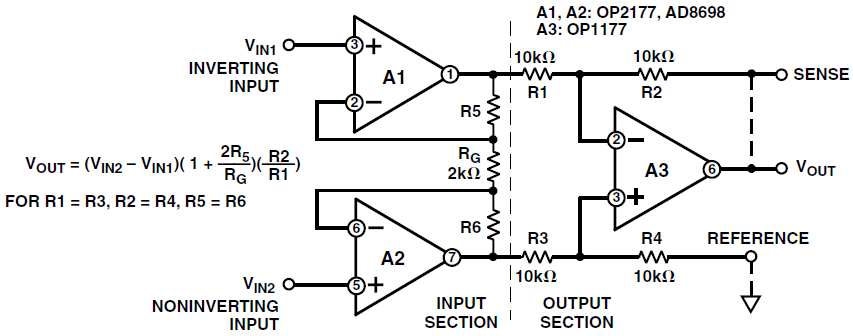
\includegraphics[width=0.8\textwidth]{Capitulo_2/Amplificador_instrumentacion.png}
  \caption{Diseño clásico de un amplificador de instrumentación con 3 amplificadores diferenciales \cite{design guide}.}
  \label{amp instrumentacion clasico} 
\end{figure}


La idea de un amplificador diferencial en un inicio podría parecer una contradicción en el sentido de que si inicialmente se disponen de dos electrodos (G1 y G2) conectados en el mismo musculo se supone ambos reciben la misma señal de entrada, así que a la salida la sumatoria de las mismas debería dar como resultado cero. \cite{EMG_instrumentation}. \\
Sin embargo es importante recordar que la acción del potencial eléctrico se debe propagar a lo largo de las fibras musculares, por lo tanto si se dispone de dos electrodos en configuración bipolar sobre el musculo la señal percibida por el G1 estará retrasada o adelantada con respecto a G2, este factor de atraso depende de la velocidad de conducción de la fibra y la distancia entre los electrodos (interelectrode distance IED), por lo que se concluye que ambos electrodos no detectan la misma señal biológica al mismo tiempo, todas las demás señales que se presenten entre los electrodos de manera simultanea serán consideradas ruido y por ende serán suprimidas por el amplificador diferencial al ser de modo común \cite{EMG_instrumentation}.

\begin{figure}[H]
  \centering
  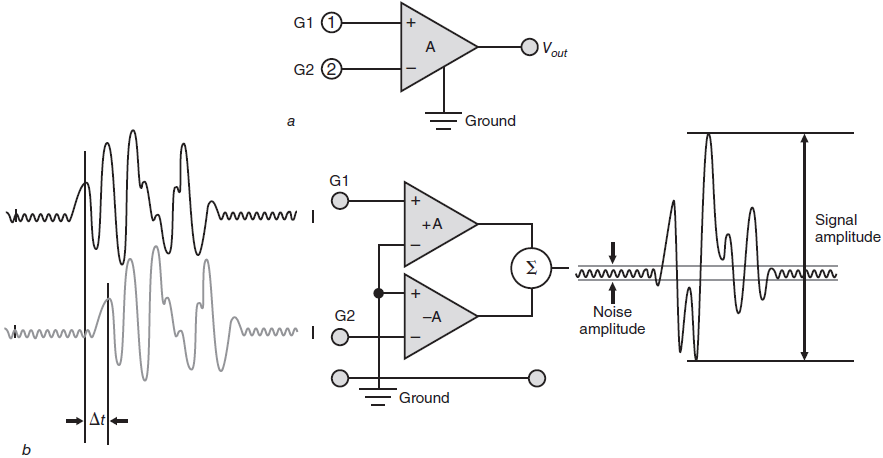
\includegraphics[width=0.8\textwidth]{Capitulo_2/signalinput.png}
  \caption{a) Los cables de G1 y G2 están conectados a una sumador, la entrada (+) es la entrada no inversora mientras que la entrada (-) es la inversora, la letra A hace referencia a la ganancia básica del amplificador. b) Este amplificador basico cuenta con dos unidades sumadoras separadas unidas a una entrada común y una salida común.}
  \label{signalinput} 
\end{figure}
%//////////////////////////////////////////////////////////////////////////
\subsubsection{Amplificador diferencial MOSFET}
%//////////////////////////////////////////////////////////////////////////
Esta porción se encargara de otorgar una impedancia de entrada alta y una impedancia de salida razonable para la etapa de ganancia, dentro de su diseño no se considero necesaria una ganancia muy grande debido a que su función principal es de acople. \\

Para la practica de laboratorio fue propuesto el diseño presentado en las figuras \ref{ampdifmosfetactloadsim} y \ref{ampdifmosfetactloadproto} sin tener en cuenta cálculos previos, esto solo se realizo con la finalidad de observar el grado de consistencia entre los resultados otorgados por la simulación y los prácticos. \\

Como resultado de las pruebas se obtuvo que la salida del amplificador diferencial era de $5 V$ DC y que era imposible poder apreciar alguna amplificación de la señal de entrada, esto puede que se deba a que el nivel DC se encontraba muy por encima saturando a los transistores de carga activa y por ende impidiendo observar algún rastro de amplificación.

\begin{figure}[H]
  \centering
  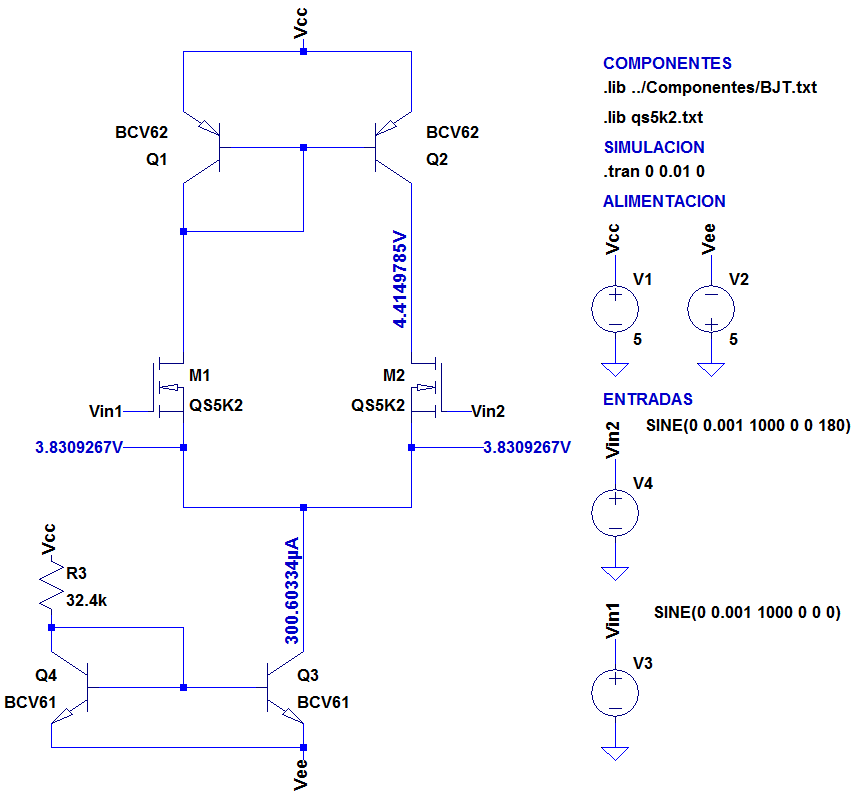
\includegraphics[width=0.6\textwidth]{Capitulo_2/ampdifmosfet.png}
  \caption{Amplificador diferencial con mosfet y espejos de corriente bipolares.}
  \label{ampdifmosfetactloadsim} 
\end{figure}

\begin{figure}[H]
  \centering
  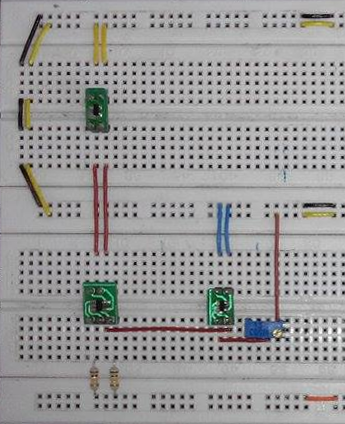
\includegraphics[width=0.5\textwidth]{Capitulo_2/pro_ampdifmosfet.png}
  \caption{Amplificador diferencial con mosfet y espejos de corriente bipolares.}
  \label{ampdifmosfetactloadproto} 
\end{figure}

Atendiendo al problema anterior se reemplaza la carga activa por una resistencias de 15 $k\Omega$ en cada rama, y la resistencia de programación de la corriente del espejo sigue siendo 32 $k\Omega$, debido a las imposibilidades impuestas por el generador de funciones, la señal de entrada se reemplaza por una de 15 $mV_{pico}$. El circuito propuesto puede observarse en la figura \ref{ampdifmosfetressim} y los resultados de su simulación en la figura \ref{sim-mosfet-indif-sinout}. Para este caso la ganancia obtenida por rama fue de 14.8 y se calculo de la siguiente manera. \\

\begin{equation}
Av=\frac{vo}{vin}=\frac{vo}{vi_1-vi_2}=\frac{444}{15-(-15)}=14.8 v/v
\end{equation}

%--------------------------------------------------------------
\begin{figure}[H]

\centering

\begin{tikzpicture}
\begin{axis}[scale=1,
    width=\textwidth,
    height=6cm,
    grid=both,
    grid style={line width=.1pt, draw=gray!10},
    major grid style={line width=.2pt,draw=gray!50},
    minor tick num=9,
    enlargelimits=false,
	title=Salida sencilla,
    xlabel= Tiempo(Seg),
	ylabel= Voltaje(V),
]
\addplot [black,very thick] table [x={time}, y={V(vin1)}] {Capitulo_2/sim-mosfet-indif-sinout.txt}; 
\addplot [red,very thick] table [x={time}, y={V(salida)}] {Capitulo_2/sim-mosfet-indif-sinout.txt}; 
\addlegendentry{Entrada}
\addlegendentry{Salida}
\end{axis}
\end{tikzpicture}

\caption{Salida sencilla referenciada a tierra del amplificador diferencial mosfet con carga resistiva y entrada diferencial}
\label{sim-mosfet-indif-sinout}

\end{figure}
%--------------------------------------------------------------
\begin{figure}[H]
  \centering
  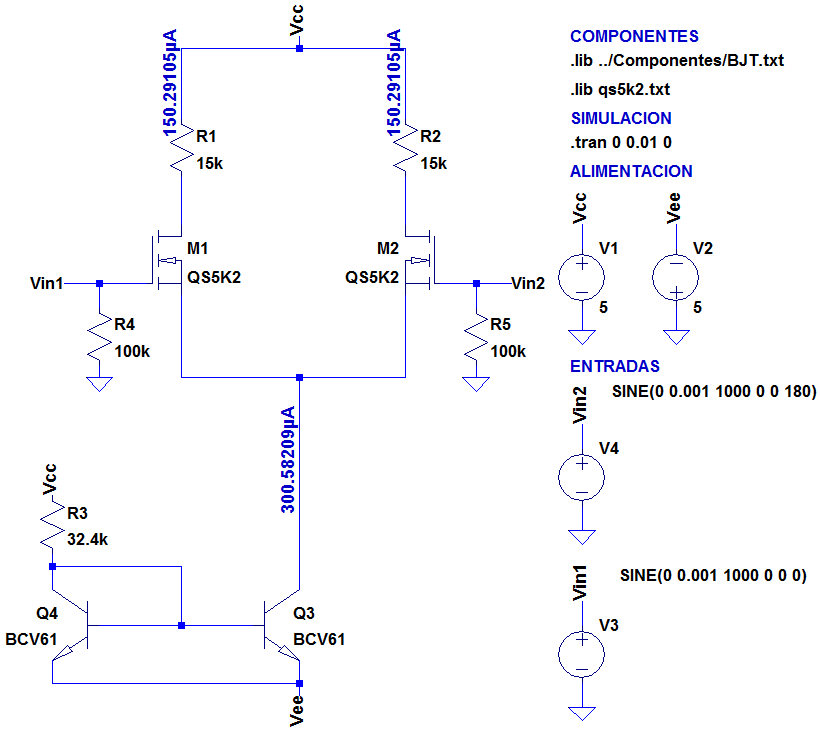
\includegraphics[width=0.6\textwidth]{Capitulo_2/ampdifmosfetres.png}
  \caption{Amplificador diferencial con mosfet y carga resistiva.}
  \label{ampdifmosfetressim}
\end{figure}

%--------------------------------------------------------------
\begin{figure}[H]

\centering

\begin{tikzpicture}
\begin{axis}[scale=1,
    width=\textwidth,
    height=6cm,
    grid=both,
    grid style={line width=.1pt, draw=gray!10},
    major grid style={line width=.2pt,draw=gray!50},
    minor tick num=9,
    enlargelimits=false,
	title=Salida diferencial,
    xlabel= Tiempo(Seg),
	ylabel= Voltaje(V),
    scaled y ticks = false,
    yticklabel style={/pgf/number format/fixed,
                     /pgf/number format/precision=3},
]
\addplot [blue,very thick] table [x={tiempo}, y={ganancia1}] {Capitulo_2/lab-mosfet-indif-sinout.txt};
\addplot [red,very thick] table [x={tiempo}, y={ganancia2}] {Capitulo_2/lab-mosfet-indif-sinout.txt};
\addlegendentry{$158\mu A$}
\addlegendentry{$190\mu A$}
\end{axis}
\end{tikzpicture}

\caption{Cambios en la magnitud de la señal de salida ante distintos valores de corriente $I_D$, al considerar ambas entradas en el amplificador diferencial.}
\label{salida-diferencial-mosfet-resistencia}

\end{figure}
%--------------------------------------------------------------

En el momento en que son realizadas las pruebas por medio de los electrodos, no se logró apreciar ninguna señal asociada a algún movimiento muscular, lo único observable era ruido, la solución inicial propuesta consiste en incrementar el valor de ganancia del amplificador MOSFET con la finalidad de lograr observar una respuesta favorable ante los estímulos musculares.\\

La ganancia por rama del amplificador diferencial como se ha mencionado anteriormente viene dada por la ecuación:

\begin{equation}
Av=\frac{1}{2}gm\cdot R_d
\end{equation}

Donde el valor de gm depende de la polarizacion del transistor y $R_d$ no puede ser muy grande debido a que su tamaño podría bajar mucho el nivel DC llegando a puntos donde no se deja una ventana de voltaje en la cual pueda ser apreciada la señal sino que todo el voltaje es consumido tanto por la resistencia como por el transistor y el espejo.

%Colocar la maxima corriente que se podria colocar sin alterar el nivel DC demasiado, la prueba en la que casi se quema el pot y que luego de cambiar las resistencias de las ramas los mejores resultados fueron obtenidos acorde al modelo original.

\textbf{Datos:}
\begin{itemize}
  \item Ganancia por rama = 14 $V/V$.
  \item Impedancia de entrada = 947 $k\Omega$.
  \item Impedancia de salida sencilla 8.43 $k\Omega$
  \item Nivel DC $\approx$ 1.12 $V$
  \item Resistencia de programación de la fuente de corriente: 24.2 $k\Omega$
  \item Corriente por rama $\approx 202 \mu A$
\end{itemize}
%//////////////////////////////////////////////////////////////////////////
\subsection{Seguidor por emisor}
%//////////////////////////////////////////////////////////////////////////
La resistencia de salida del seguidor por emisor fue de $340 \Omega$ mientras que su impedancia de entrada resulto de $483 k\Omega$ la idea original consistia en implementar un divisor de voltaje en la entrada del amplificador con la finalidad de ajustar el nivel de voltaje DC a la entrada, sin embargo después de realizar las pruebas en el laboratorio se considero que ajustar el voltaje DC a la entrada no era necesario, primero por el hecho de que el condensador de acople permitía separar el nivel DC de ambas etapas y segundo debido a que solo bastaba una resistencia que funcionase como un lazo de corriente entre la base del transistor y la tierra con la finalidad de que la corriente necesaria para polarizar el transistor proviniese de esta conexión mas no de la señal que se desea seguir. \\

\textbf{Datos:}
\begin{itemize}
\item Impedancia de entrada = $483 k\Omega$
\item Impedancia de salida  = $340 \Omega$.
\item Nivel DC $\approx$ -2.70 $V$
\item Resistencia de programación de la fuente de corriente: 20.87 $k\Omega$
\item Corriente de polarización $\approx 467 \mu A$
\end{itemize}

%//////////////////////////////////////////////////////////////////////////
\subsection{Amplificador diferencial BJT}
%//////////////////////////////////////////////////////////////////////////
El amplificador diferencial presentado a continuacion fue desarrollado con la finalidad de observar la equivalencia entre las simulaciones y el montaje físico de los transistores.
Primero se estableció una ganancia por rama de 45 a partir de una corriente en el colector de los transistores QS5W1 haciendo uso de la siguiente ecuación.

\begin{align} \label{vfs}
A_d  &= \frac{1}{2}\frac{Ic_Q}{V_t}R_c \\ 
Ic_Q &= \frac{2A_d\cdot V_t}{R_c} = \frac{2\cdot45\cdot0.025}{15000} = 150 \mu A
\end{align}

\begin{figure}[H]
  \centering
  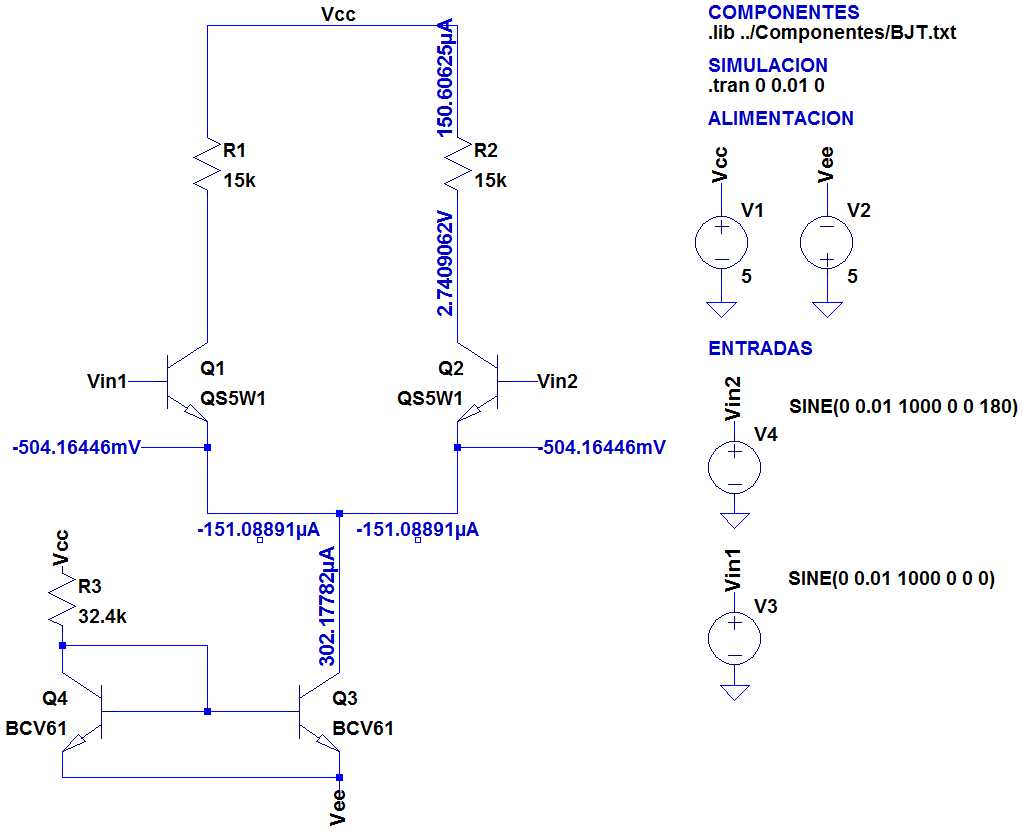
\includegraphics[width=0.8\textwidth]{Capitulo_2/ampdifbjt.png}
  \caption{Amplificador diferencial con transistores bipolares.}
  \label{ampdifbjt} 
\end{figure}

\begin{figure}[H]
  \centering
  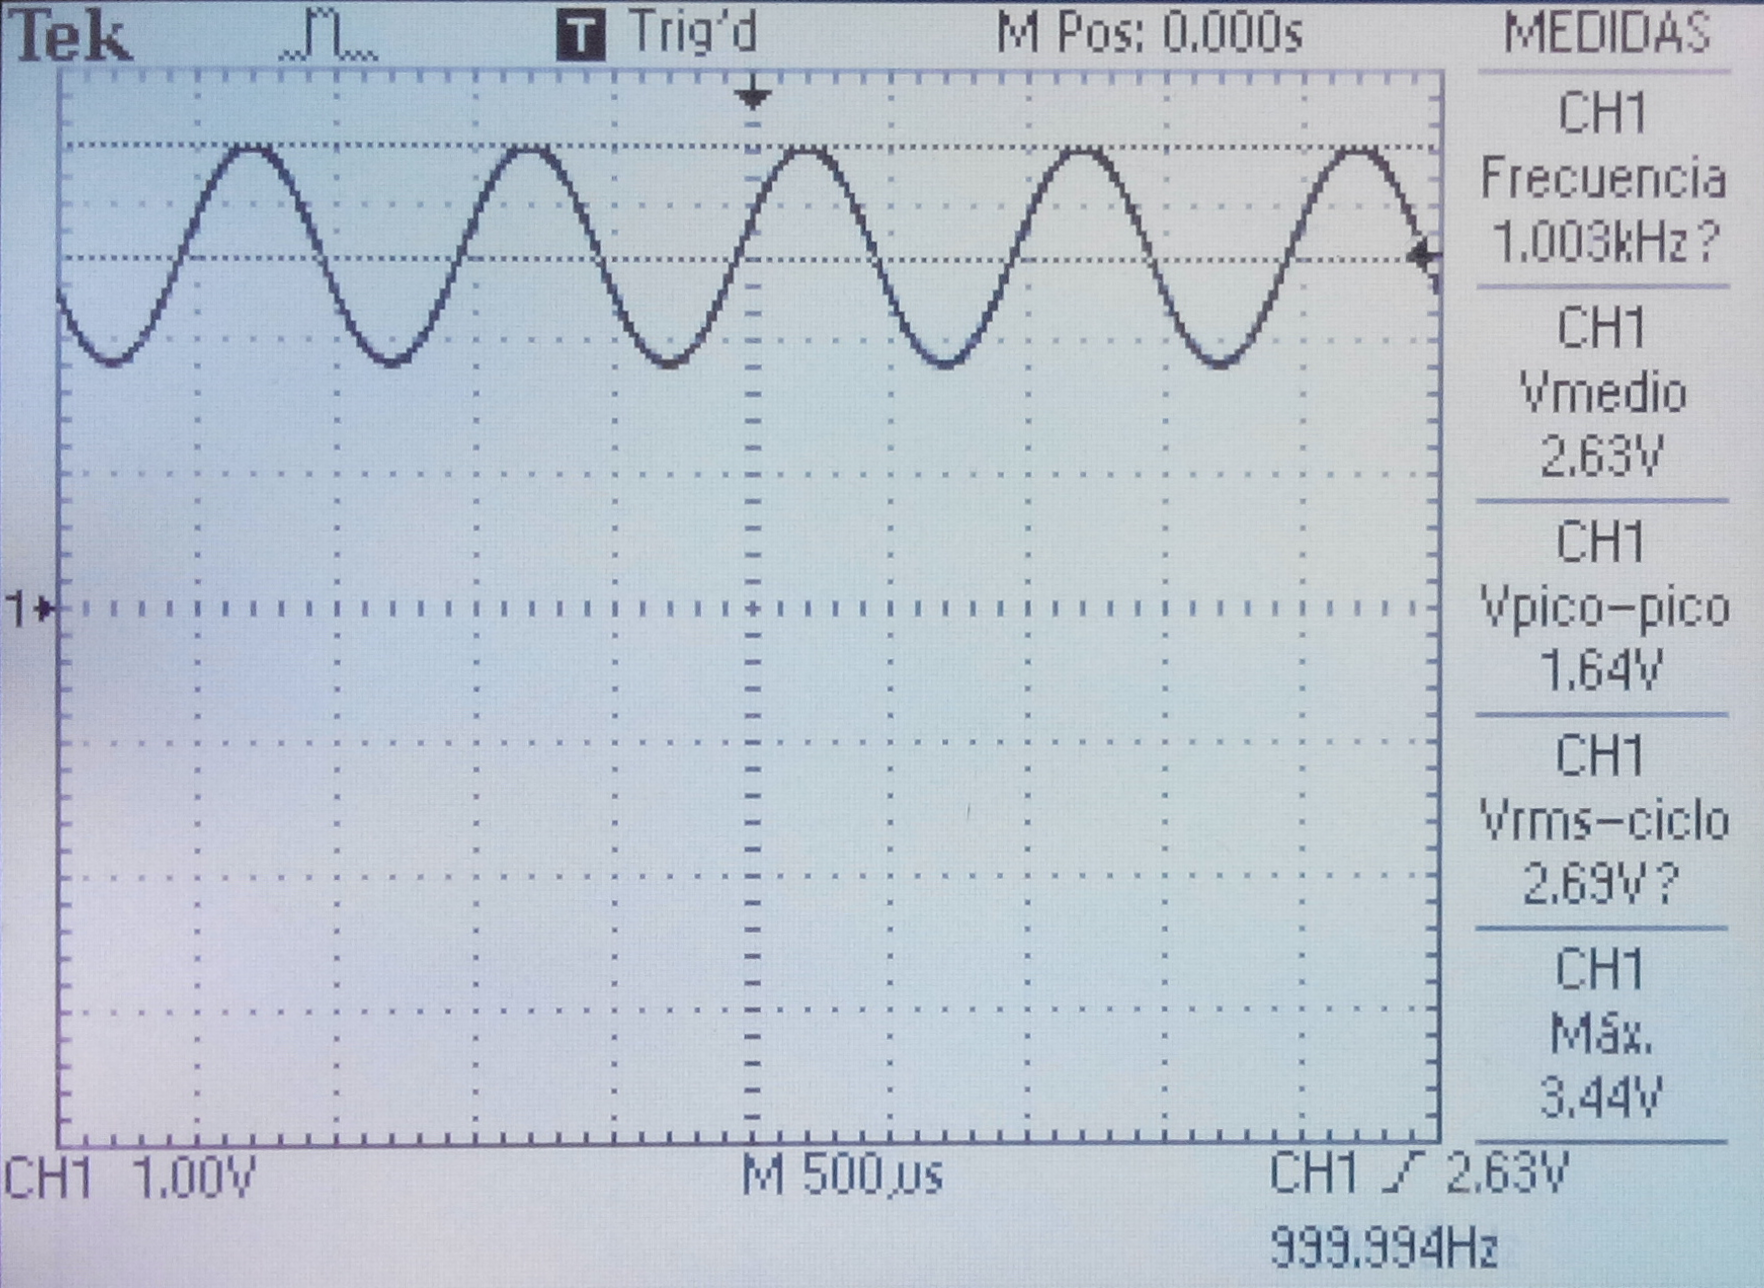
\includegraphics[width=0.8\textwidth]{Capitulo_2/lab_ampdifbjt.png}
  \caption{Amplificador diferencial con transistores bipolares.}
  \label{ampdifbjt} 
\end{figure}

\textbf{Datos:}
\begin{itemize}
\item Ganancia por rama = 1.48 $V$/0.02 $V$  = 74 $V/V$.
\item Voltaje resistencia rama izquierda: 3.434 $V$.
\item Voltaje resistencia rama derecha: 3.472 $V$.
\item Impedancia de entrada diferencial: $1.929 k\Omega$, despues de reemplazar la resistencia conectada en la base por una de 330 $k\Omega$ originalmente tenia una de 160 $k\Omega$ lo que daba como resultado una impedancia de entrada de $1.360 k\Omega$.
\item Impedancia de salida por rama $11.88 k\Omega$.
\item Resistencia de programación de la fuente de corriente: 24,9 $k\Omega$
\item Corriente por rama $\approx 195 \mu A$
\end{itemize}

\textbf{Nota:} Algunos de los parámetros cambiaron al momento de realizar las mediciones con el voltímetro, situación que no es muy favorable. 



%IDEAS
% http://masteringelectronicsdesign.com/how-to-derive-the-instrumentation-amplifier-transfer-function/
% http://www.circuitstoday.com/instrumentation-amplifier
% http://www.electronicshub.org/instrumentation-amplifier-basics-applications/





\section{Filtro Pasabanda }

En el desarrollo del electromiógrafo, es necesaria la implementación de un filtro pasabanda ya que las señales EMG se encuentran en un intervalo aproximadamente entre los 50 Hz y los 5 kHz, como se observaba en el capítulo 2. De no realizarse esta etapa, sería posible obtener señales de otros intervalos como las ECG o AAP.\\

Se propone el circuito que se muestra en la figura \ref{bandpass}, en el cual se muestra una configuración de seguidor de emisor para la implementación del mencionado filtro. La respuesta en frecuencia del circuito se puede apreciar en el diagrama de Bode que de muestra en la figura \ref{bode_bandpass}. 

\begin{figure}[H]
  \centering
  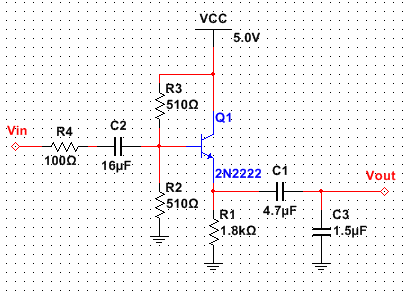
\includegraphics[width=0.8\textwidth]{Capitulo_2/bandpass_filt.png}
  \caption{Filtro Pasabanda EMG}
  \label{bandpass}
\end{figure}

\begin{figure}[H]
  \centering
  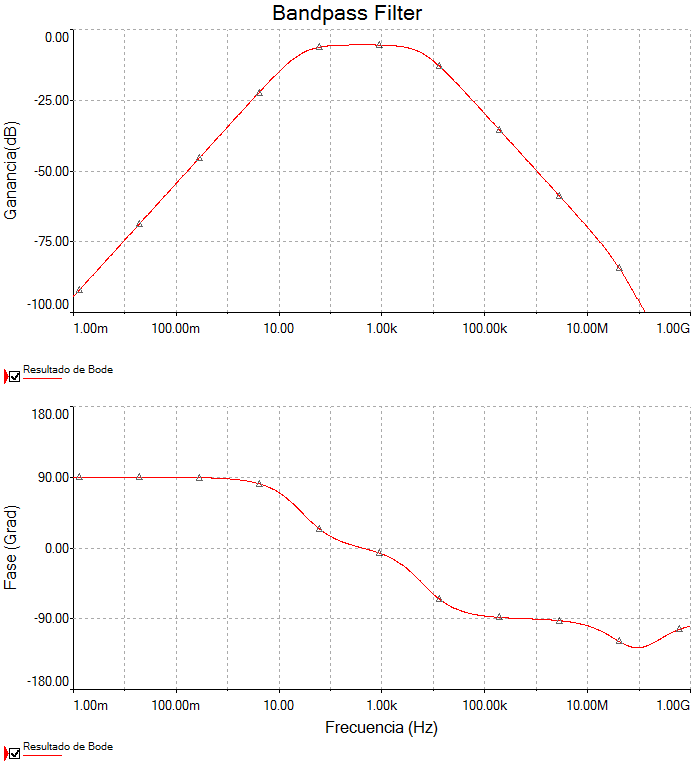
\includegraphics[width=0.9\textwidth]{Capitulo_2/bode_bandpass.png}
  \caption{Diagrama de Bode Filtro Pasabanda EMG}
  \label{bode_bandpass}
\end{figure}

\section{Rectificador de Onda Completa de Precisión}

Una vez filtrada la señal EMG obtenida en la etapa anterior, es necesario realizar una rectificación de onda completa. Inicialmente se tomará como referencia el modelo de rectificador propuesto en la figura \ref{rect_opamp}. La señal de salida de la figura \ref{osc_rect_opamp} corresponde a una señal sinusoidal rectificada de $2V_p$ y $1kHz$ de frecuencia.


\begin{figure}[H]
  \centering
  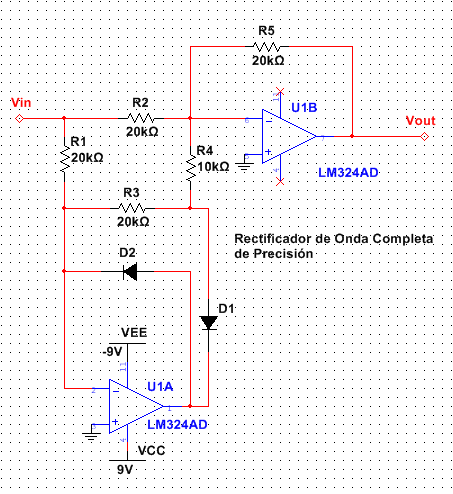
\includegraphics[width=0.65\textwidth]{Capitulo_2/op_amp_rectifier.png}
  \caption{Rectificador de onda Completa de Precisión utilizando Amplificadores Operacionales}
  \label{rect_opamp}
\end{figure}


\begin{figure}[H]
  \centering
  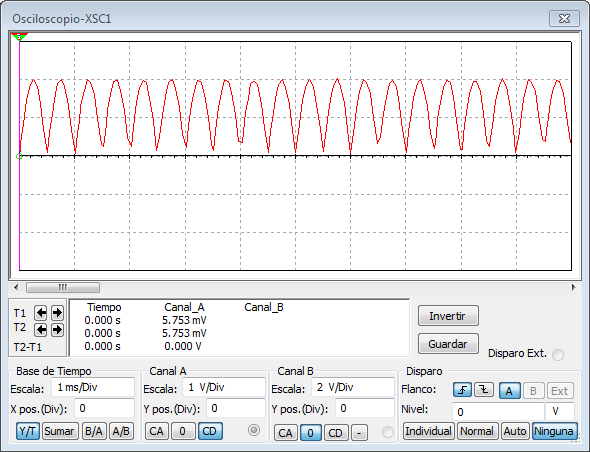
\includegraphics[width=0.6\textwidth]{Capitulo_2/osc_op_amp_rectifier.png}
  \caption{Señal de Salida Rectificador de onda Completa de Precisión utilizando Amplificadores Operacionales}
  \label{osc_rect_opamp}
\end{figure}